\chapter{Opis doświadczenia}
Przeprowadzone doświadczenie polega na porównaniu dostępnych w środowisku Microsoft Azure algorytmów klasyfikacji danych dwu-klasowych wraz z algorytmem stworzonym na potrzeby pracy inżynierskiej o tytule ''\textit{Wykorzystanie algorytmów genetycznych w systemach wykrywania intruzów w sieciach komputerowych}''\cite{Blyszcz2022} oraz z algorytmem DANet\cite{Chen2022}. Doświadczenie przebiegało według \refsource{schematu}{fig:sch-prac}.

\begin{figure}[H]
    \centering
    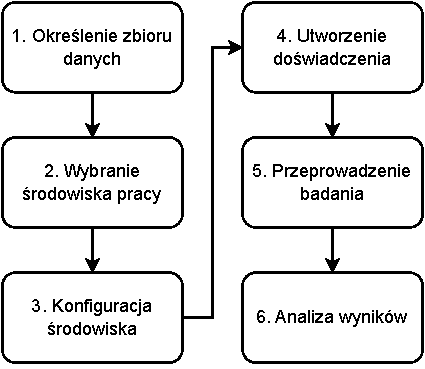
\includegraphics[width=0.5\textwidth]{images/schemat_pracy}
    \captionsource{Schemat przebiegu doświadczenia}{Opracowanie własne}
    \label{fig:sch-prac}
\end{figure}

\section{Dane}
Zbiór danych został przygotowany przez Kanadyjski Instytut Cyberbezpieczeństwa działający przy Uniwersytecie Nowy Brunszwik za pomocą narzędzia CICFlowMeter\cite{Ahlashkari2022}. Zbiór zawiera 79 cech ruchu sieciowego do których zaliczyć można: etykietę, czas trwania przesyłu, minimalną długość pakietu zwrotnego, maksymalną długość pakietu zwrotnego, port docelowy, długość pakietów. Zbiór pozwala na określenie czy ruch sieciowy jest życzliwy \trans{ang. BENING}, czy nieżyczliwy (różne możliwe formy ataku na sieć). Dodatkowo zbiór został podzielony na pięć dni roboczych: poniedziałek 3.07.2017 - piątek 7.07.2017. Dane z poniedziałku zawierają jedynie ruch życzliwy, zaś w pozostałe dni zostały zasymulowane ataki na sieć komputerową\cite{Blyszcz2022, unbkaggle}.

\section{Środowisko programistyczne}
Jako środowisko programistyczne zostało wybrane Azure Machine Learning Studio z powodu możliwości uniezależnienia obliczeń od komputera lokalnego, dodatkowo platforma umożliwia łatwy sposób na tworzenie skomplikowanych potoków zadań, które składają się z komponentów wielokrotnego użytku. Każdy komponent uruchamia się w środowisku odizolowanym od pozostałych operacji. Dzieje się tak dzięki wykorzystaniu wielo węzłowych klastrów obliczeniowych, bazujących na oprogramowaniu Docker, klastry te mogą skalować się w zależności od potrzeb oraz dostępnej jednostki\cite{MicrosoftLearn2023}.
\\ \\
Całe doświadczenie zostało odwzorowane w graficznym potoku narzędzia ''\textit{Projektant}'' oraz przedstawione na \refsource{zdjęciu}{fig:pipeline}.
\begin{landscape}
\begin{figure}[H]
    \centering
    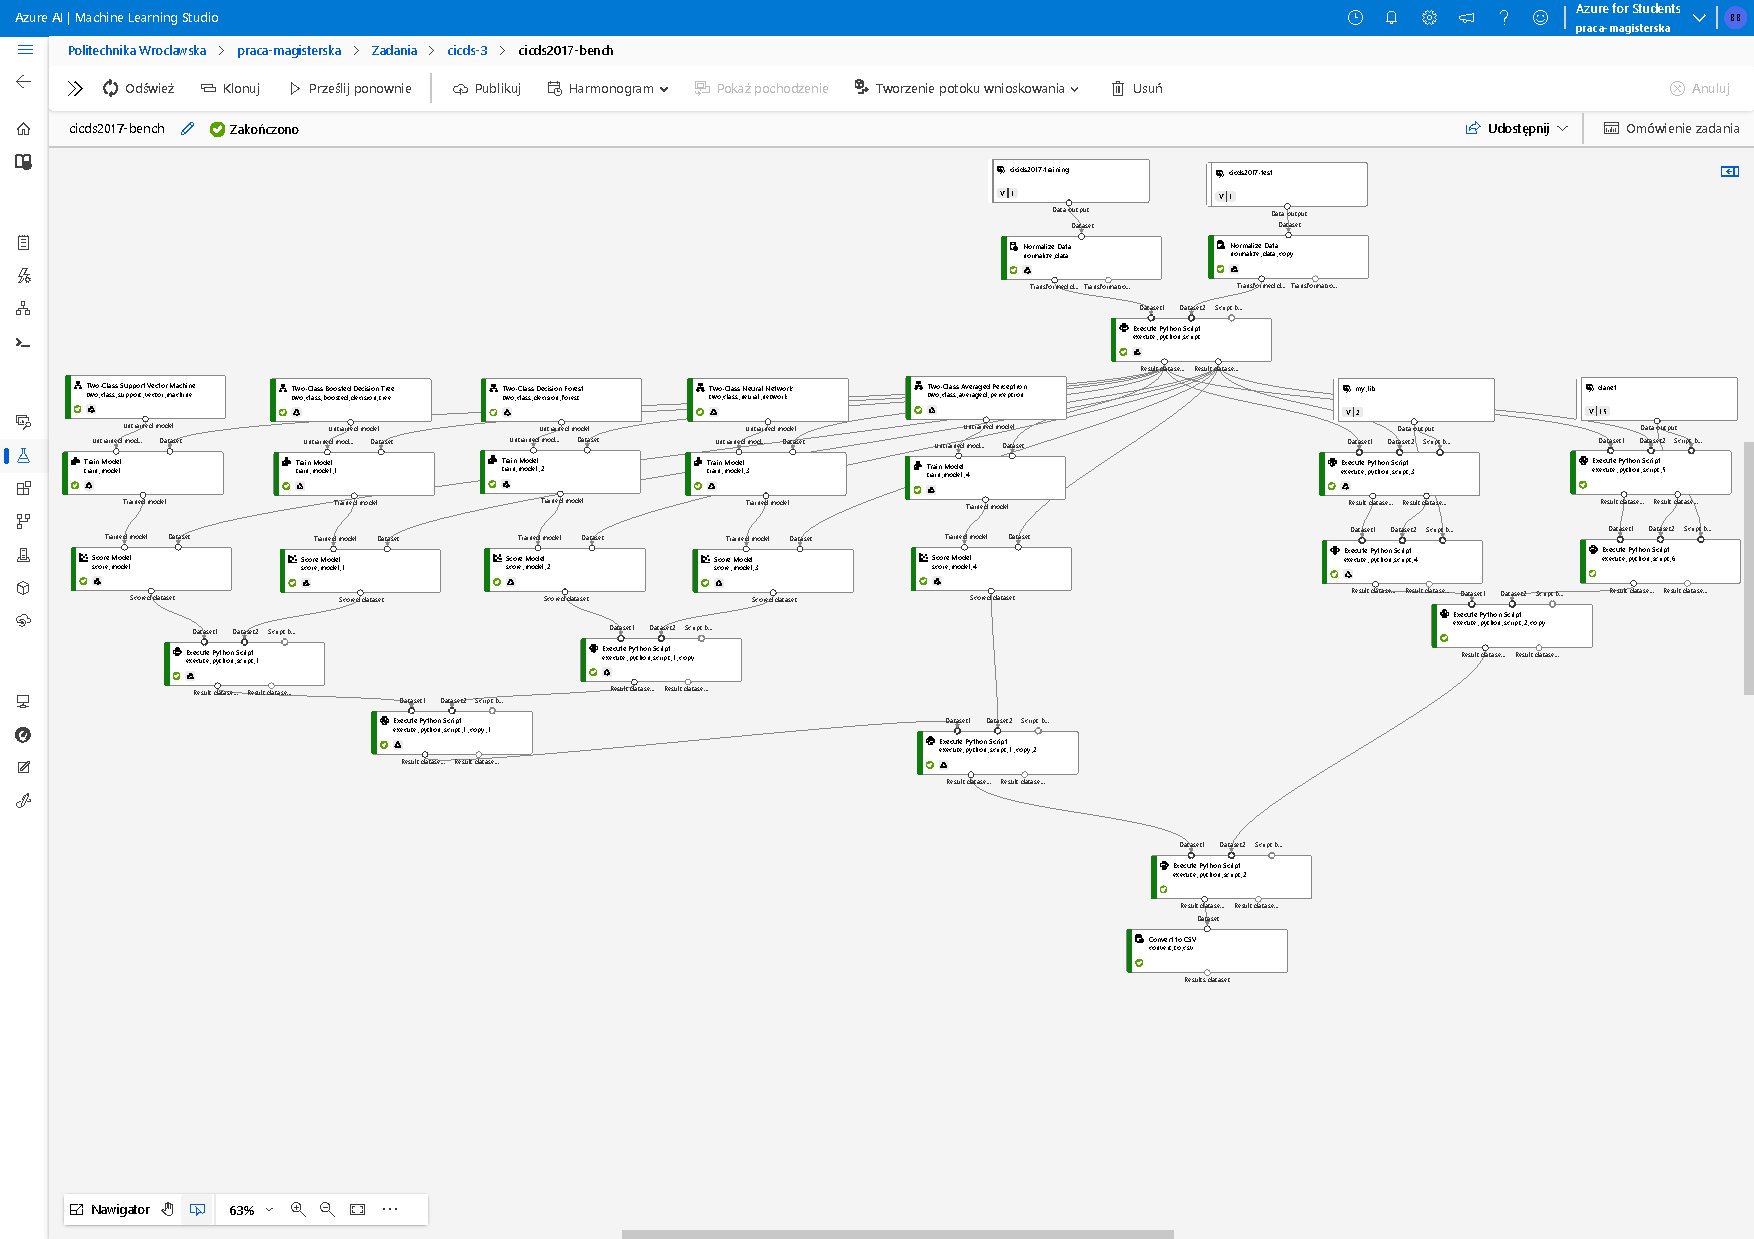
\includegraphics[height=0.95\textwidth]{images/pipeline}
    \captionsource{Potok zadań}{Opracowanie własne}
    \label{fig:pipeline}
\end{figure}
\end{landscape}

\section{Algorytmy}

\subsection{Two-Class Support Vector Machine}
\subsection{Two-Class Boosted Decision Tree}
\subsection{Two-Class Decision Forest}
\subsection{Two-class Neural Network}
\subsection{Two-Class Average Perceptron}
\subsection{Autorskie rozwiązanie}
\subsection{DANET}



